%% Real book exercises, Lectures 1--5: all 50 items.
%% Layout: preamble and blocks in Listas/lista-reais-lectures-01-05/ (order in order.md).
%% Compile from Listas/: pdflatex lista-reais-lectures-01-05.tex (2x); pdffonts lista-reais-lectures-01-05.pdf (all Type 1).
\documentclass[11pt,a4paper]{article}
\newcommand{\listatema}{Real Book Exercises, Lectures 1--5}
% =============================================================================
% Shared preamble of the real-exercise list for Lectures 1--5 (real schedule).
% Input by Listas/lista-reais-lectures-01-05.tex (all blocks) and by
% Listas/lista-reais-lecture-0N.tex (one block). The driver defines \listatema before
% \input-ing this file; a per-lecture driver then sets \perlecturetrue and \blockoffset
% (number of items in the earlier blocks) so items are numbered 1--10 and also cite their
% number in the combined list. Rules: rules/00_estilo_avaliacao.md §5.
% =============================================================================
\usepackage[utf8]{inputenc}
\usepackage[T1]{fontenc}
\usepackage{lmodern}   % Type 1 vector fonts (replaces PK bitmaps)
\usepackage{cmap}      % ToUnicode CMap -> copyable text and accents
\usepackage[english]{babel}
\usepackage{amsmath,amssymb,amsfonts,mathtools}
\usepackage[a4paper,margin=2.2cm]{geometry}
\usepackage{enumitem}
\usepackage{fancyhdr}
\usepackage{xcolor}
\usepackage{microtype}
\usepackage{booktabs}
\usepackage{graphicx}
\usepackage{array}
\usepackage{needspace}

\newcommand{\disciplina}{Economia das Organizações e dos Incentivos --- MPE Insper}
\newcommand{\espacoresol}{3.5cm}   % height of the resolution space after each exercise

\pagestyle{fancy}\fancyhf{}
\lhead{\footnotesize\disciplina}
\rhead{\footnotesize \listatema}
\cfoot{\footnotesize\thepage}
\renewcommand{\headrulewidth}{0.3pt}
\setlength{\headheight}{14pt}

\setlist{topsep=2pt,itemsep=2pt}
\setlength{\parindent}{0pt}
\setlength{\parskip}{4pt}
\newcounter{questao}

% Per-lecture mode: items numbered 1--10, with their number in the combined list.
\newif\ifperlecture
\newcommand{\blockoffset}{0}
\newcommand{\rownum}[1]{\ifperlecture\the\numexpr#1-\blockoffset\relax\ (#1)\else#1\fi}

% Block header: number, lecture title, coverage.
\newcommand{\bloco}[3]{\bigskip\noindent
  {\large\bfseries\color{blue!55!black}Block #1 --- #2}\hfill\textit{(#3)}\par
  \noindent\rule{\linewidth}{0.3pt}\smallskip}
% Exercise header: [#1] difficulty 1--5, #2 short name, #3 level, #4 source line.
\newcommand{\exercicio}[4][]{\needspace{12\baselineskip}\refstepcounter{questao}\medskip\noindent
  \textbf{Exercise \thequestao.}\ifperlecture~{\small(item
  \the\numexpr\value{questao}+\blockoffset\relax\ of the combined list)}\fi~\textit{#2}%
  % keeps the [level; difficulty] tag whole, right-aligned on the last line (TeXbook \signed)
  {\unskip\nobreak\hfil\penalty50\hskip1em\hbox{}\nobreak\hfill\mbox{\small[#3; difficulty #1/5]}}\par
  \noindent{\small\color{black!70}\textbf{Source.} #4}\par\smallskip}
% Material an exercise refers to, copied in under its own source line.
\newenvironment{referencia}[1]{\par\smallskip\noindent
  \begin{minipage}{\linewidth}\small\leftskip=1.2em
  \noindent\textbf{Referenced material.} {\color{black!70}\textbf{Source.} #1}\par\smallskip}%
  {\end{minipage}\par}
% Book's exercise label inside the statement, e.g. "4.5".
\newcommand{\rot}[1]{\textbf{#1}\quad}
\newcommand{\resolespaco}{\par\textit{Resolution:}\vspace{\espacoresol}\par}
% Payoff matrix: #1 row-player label, #2 column-player label, #3 inner tabular.
\newcommand{\jogo}[3]{\begin{center}\begin{tabular}{@{}r@{\hspace{6pt}}c@{}}
  & #2\\[2pt] #1 & #3\end{tabular}\end{center}}
\newcommand{\hd}[1]{\multicolumn{1}{c}{#1}}
\newenvironment{partes}{\begin{enumerate}[label=\alph*.,leftmargin=2em]}{\end{enumerate}}

% ----------------------------------------------------------------------------- front page
\newcommand{\titulo}{\begin{center}
  {\Large\bfseries \disciplina}\\[2pt]
  {\large Exercise List: \listatema}
\end{center}}

\newcommand{\howtouse}{{\small\noindent\textbf{How to use this list.} Every exercise below is a
real exercise from one of the course books, reproduced verbatim: the source line gives author,
book, chapter, exercise, the printed page and, in brackets, the page your PDF viewer shows for the
file in \texttt{Livros/}, and whether the source gives the answer. Muñoz-Garcia \& Toro-Gonzalez
print a worked answer right after each exercise; MWG answers are in the MWG solutions manual in
\texttt{Livros/}; Tadelis, Gibbons and Cabral give no answer in the book. When an exercise refers
to a model, game or figure stated elsewhere in its book, that material is copied into the same
block under ``Referenced material'', so every exercise can be solved where it is printed. There is
one block per lecture of the real schedule. Each block has ten exercises in strictly rising
difficulty, rated from 1 (apply a definition) to 5 (graduate level) next to each heading: three
foundations, five exam level, two advanced. Try each exercise in the space provided before opening
the book's answer.\par}}

% Selection table; #1 = the rows of one block (\rowsi ... \rowsv).
\newcommand{\selectiontable}[1]{\begin{center}
\footnotesize
\setlength{\tabcolsep}{2.8pt}
\begin{tabular}{@{}c r l r l >{\raggedright\arraybackslash}p{4.0cm} c c@{}}
\toprule
Block & \# & Source & p. [PDF] & Level & What it trains & Diff. & Answer \\
\midrule
#1
\bottomrule
\end{tabular}
\end{center}}

\newcommand{\tablenote}{{\footnotesize \ifperlecture \#: item number in this lecture's list,
then its number in the combined list (\texttt{lista-reais-lectures-01-05.pdf}) in brackets.
\fi Items not in the list for Lectures 1--4 (\texttt{lista-reais-lectures-01-04.tex}) are marked:
$^\dagger$\,added in the 30-item version, $^\ddagger$\,added in the 50-item version. Every other
item is reused from that list with its statement unchanged, some in a different block or position.
``Diff.'': difficulty from 1 (apply a definition) to 5 (graduate level). Pages: printed page, then
the PDF viewer page in brackets (offsets in \texttt{Livros/book-registry.json}; MWG is a
two-pages-per-sheet scan). ``Answer'': \emph{book} = worked answer printed after the exercise;
\emph{manual} = MWG solutions manual in \texttt{Livros/}; \emph{none} = no answer in the book.
Books: Tadelis (2013), \emph{Game Theory: An Introduction}; Gibbons (1992), \emph{Game Theory for
Applied Economists}; Muñoz-Garcia \& Toro-Gonzalez (2019), \emph{Strategy and Game Theory: Practice
Exercises with Answers}, 2nd ed.; Mas-Colell, Whinston \& Green (1995), \emph{Microeconomic Theory}
(MWG); Cabral (2017), \emph{Introduction to Industrial Organization}, 2nd ed.\par}}

\newcommand{\rowsi}{%
L1 & \rownum{1} & Tadelis 4.5 & 77 [96] & Found. & IESDS round by round, $3\times3$ matrix & 1 & none \\
   & \rownum{2} & Muñoz-Garcia Ch.~1 Ex.~13$^\ddagger$ & 26 [39] & Found. & Dominant and dominated strategies, then IDSDS & 1 & book \\
   & \rownum{3} & Gibbons 1.2 & 48 [56] & Found. & IESDS, then pure Nash equilibria & 2 & none \\
   & \rownum{4} & Tadelis 4.1$^\ddagger$ & 76 [95] & Exam & Proof: a strictly dominant-strategy equilibrium is unique & 2 & none \\
   & \rownum{5} & Muñoz-Garcia Ch.~1 Ex.~12 & 23 [36] & Exam & Rationality vs.\ common knowledge of it & 2 & book \\
   & \rownum{6} & Tadelis 4.7 & 77--78 [96--97] & Exam & Story to matrix, then elimination & 3 & none \\
   & \rownum{7} & Tadelis 4.3$^\ddagger$ & 76 [95] & Exam & Discrete first-price auction: matrix, IESDS & 3 & none \\
   & \rownum{8} & Tadelis 4.6 & 77 [96] & Exam & IESDS with continuous strategies & 4 & none \\
   & \rownum{9} & MWG 8.B.4$^\ddagger$ & 262 [142] & Adv. & Proof: the order of strict deletion does not matter & 4 & manual \\
   & \rownum{10} & MWG 8.B.5 & 262 [142] & Adv. & Cournot by IESDS: two firms vs.\ three & 5 & manual \\}
\newcommand{\rowsii}{%
L2 & \rownum{11} & Tadelis 5.6 & 96 [115] & Found. & Hawk-dove: matrix, pure equilibria & 1 & none \\
   & \rownum{12} & Muñoz-Garcia Ch.~2 Ex.~2$^\ddagger$ & 41 [54] & Found. & Battle of the sexes: pure equilibria & 1 & book \\
   & \rownum{13} & Muñoz-Garcia Ch.~3 Ex.~1 & 86--87 [99--100] & Found. & Chicken: pure and mixed equilibria & 2 & book \\
   & \rownum{14} & Gibbons 1.12$^\ddagger$ & 51 [59] & Exam & A mixed equilibrium by indifference & 2 & none \\
   & \rownum{15} & Tadelis 5.8 & 96--97 [115--116] & Exam & Cournot with $n$ firms; competitive limit & 3 & none \\
   & \rownum{16} & Gibbons 1.6 & 49 [57] & Exam & Cournot, asymmetric costs; corner case & 3 & none \\
   & \rownum{17} & Gibbons 1.7$^\ddagger$ & 49--50 [57--58] & Exam & Homogeneous Bertrand: $p_1 = p_2 = c$ is the unique equilibrium & 3 & none \\
   & \rownum{18} & Tadelis 6.8 & 125 [144] & Exam & Three-player entry; symmetric mixing & 4 & none \\
   & \rownum{19} & MWG 8.D.2$^\ddagger$ & 263 [142] & Adv. & Proof: a unique IESDS survivor is a Nash equilibrium & 4 & manual \\
   & \rownum{20} & MWG 8.D.6 & 264 [143] & Adv. & A mixed equilibrium exists in every $2\times2$ game & 5 & manual \\}
\newcommand{\rowsiii}{%
L3 & \rownum{21} & Tadelis 7.1$^\ddagger$ & 147 [166] & Found. & Counting pure strategies over information sets & 1 & none \\
   & \rownum{22} & Muñoz-Garcia Ch.~4 Ex.~3 & 160 [172] & Found. & Sequential prisoner's dilemma & 1 & book \\
   & \rownum{23} & Tadelis 7.2$^\dagger$ & 147 [166] & Found. & Story to tree; strategies; an ``unappealing'' Nash equilibrium & 2 & none \\
   & \rownum{24} & Tadelis 8.5$^\dagger$ & 170 [189] & Exam & A simultaneous game behind an adoption choice: SPE & 3 & none \\
   & \rownum{25} & Tadelis 8.10 & 172 [191] & Exam & Subgames with a simultaneous stage & 3 & none \\
   & \rownum{26} & Tadelis 7.4$^\ddagger$ & 148 [167] & Exam & Four-move centipede: strategies, Nash equilibria, outcomes & 3 & none \\
   & \rownum{27} & Tadelis 7.9$^\ddagger$ & 149--150 [168--169] & Exam & A move of Nature and an information set & 4 & none \\
   & \rownum{28} & Tadelis 7.10$^\dagger$ & 150 [169] & Exam & Mixed vs.\ behavioral strategies; perfect recall & 4 & none \\
   & \rownum{29} & MWG 9.B.4$^\ddagger$ & 302 [162] & Adv. & Proof: unique SPNE payoffs in zero-sum games of perfect information & 4 & manual \\
   & \rownum{30} & Gibbons 2.1 & 130 [137] & Adv. & Rotten Kid theorem (continuous actions) & 5 & none \\}
\newcommand{\rowsiv}{%
L4 & \rownum{31} & Gibbons 2.12$^\dagger$ & 135 [142] & Found. & Strategy, subgame and SPE in a repeated game & 1 & none \\
   & \rownum{32} & Tadelis 7.6$^\ddagger$ & 148--149 [167--168] & Found. & Entry game: payoffs from preferences, all Nash equilibria & 1 & none \\
   & \rownum{33} & Tadelis 8.8 & 171--172 [190--191] & Found. & Entry deterrence: a non-credible threat & 2 & none \\
   & \rownum{34} & Tadelis 8.6$^\dagger$ & 170--171 [189--190] & Exam & Sunk investment before Cournot; threshold $F^*$ & 3 & none \\
   & \rownum{35} & Muñoz-Garcia Ch.~4 Ex.~11$^\ddagger$ & 180 [192] & Exam & Stackelberg, asymmetric costs; vs.\ monopoly, Cournot, Bertrand & 3 & book \\
   & \rownum{36} & Tadelis 8.11$^\ddagger$ & 172--173 [191--192] & Exam & Sequential vetoes; Nash equilibria that are not SPE; removing an option & 3 & none \\
   & \rownum{37} & Tadelis 8.4$^\dagger$ & 170 [189] & Exam & Leader, two followers: subgames; a Nash equilibrium that is not SPE & 4 & none \\
   & \rownum{38} & Tadelis 8.13 & 173--174 [192--193] & Exam & Hold-up; a posted price as commitment & 4 & none \\
   & \rownum{39} & Tadelis 8.7$^\ddagger$ & 171 [190] & Adv. & Credibility of suing; design of the legal system & 4 & none \\
   & \rownum{40} & MWG 9.B.5$^\dagger$ & 302 [162] & Adv. & Observation, multiple SPNE, when moving first pays & 5 & manual \\}
\newcommand{\rowsv}{%
L5 & \rownum{41} & Cabral 7.13$^\dagger$ & 182 [194] & Found. & Finitely repeated PD unravels & 1 & none \\
   & \rownum{42} & Tadelis 10.2$^\dagger$ & 215 [234] & Found. & Grim trigger; threshold $\delta$ for two paths & 2 & none \\
   & \rownum{43} & Muñoz-Garcia Ch.~6 Ex.~1$^\ddagger$ & 274 [285] & Found. & One-, two- and ten-period punishments & 2 & book \\
   & \rownum{44} & Muñoz-Garcia Ch.~6 Ex.~9$^\dagger$ & 305 [316] & Exam & Feasible, individually rational payoffs; folk theorem & 3 & book \\
   & \rownum{45} & Tadelis 10.3$^\ddagger$ & 215--216 [234--235] & Exam & Length-$T$ punishments: $\delta_1$ vs.\ $\delta_2$ & 3 & none \\
   & \rownum{46} & Tadelis 9.1 & 186--187 [205--206] & Exam & Stage game played twice: all SPE, carrot and stick & 4 & none \\
   & \rownum{47} & Gibbons 2.11$^\ddagger$ & 135 [142] & Exam & A non-Nash first-stage payoff in a twice-played game & 4 & none \\
   & \rownum{48} & Tadelis 11.5 & 236--237 [255--256] & Exam & Three periods with $\delta_1\neq\delta_2$ & 4 & none \\
   & \rownum{49} & Tadelis 10.7$^\ddagger$ & 217--218 [236--237] & Adv. & Quality: ten days vs.\ forever, in parameters & 4 & none \\
   & \rownum{50} & Gibbons 2.20$^\dagger$ & 137--138 [144--145] & Adv. & Rubinstein strategies are an SPE (one-stage deviations) & 5 & none \\}

% Difficulty path: what makes each block's last item hard.
\newcommand{\pathi}{\textbf{Lecture 1}: from one $3\times3$ elimination (1) through two short proofs
about dominance (Tadelis 4.1, MWG 8.B.4) to MWG 8.B.5 (5), where elimination over a continuum of
quantities must be shown to converge with two firms and to stall with three.}
\newcommand{\pathii}{\textbf{Lecture 2}: from writing a matrix (1) through the Bertrand uniqueness
proof and MWG 8.D.2 to MWG 8.D.6 (5), a proof that every $2\times2$ game, with arbitrary payoffs,
has a mixed-strategy equilibrium.}
\newcommand{\pathiii}{\textbf{Lecture 3}: from counting strategies (1) through Nature, imperfect
recall and the zero-sum proof (MWG 9.B.4) to Gibbons 2.1 (5), a proof with general concave income
and utility functions and continuous actions.}
\newcommand{\pathiv}{\textbf{Lecture 4}: from definitions (1) through entry, Stackelberg, hold-up and
the legal-system game (Tadelis 8.7) to MWG 9.B.5 (5), a five-part general-payoff argument on
strategy counts, multiple SPNE and when moving first guarantees the simultaneous-move payoff, with
counterexamples.}
\newcommand{\pathv}{\textbf{Lecture 5}: from unraveling (1) through punishments of finite length,
carrot and stick and the both-horizons bar game (Tadelis 10.7) to Gibbons 2.20 (5), a proof that
Rubinstein's stationary strategies are a Nash equilibrium and are subgame-perfect, checking every
history of an infinite game.}


\begin{document}
\titulo
\howtouse

\medskip
{\small\noindent\textbf{Difficulty path} (what makes each block's last items hard):
\begin{itemize}[leftmargin=1.4em,itemsep=0pt]
\item \pathi
\item \pathii
\item \pathiii
\item \pathiv
\item \pathv
\end{itemize}\par}

\medskip
{\small\noindent\textbf{Selection tables} (one per lecture, next pages).\par}
\tablenote

\newpage
\selectiontable{\rowsi}
\selectiontable{\rowsii}
\selectiontable{\rowsiii}
\selectiontable{\rowsiv}
\selectiontable{\rowsv}

\newpage
% Block 1 of lista-reais-lectures-01-05 (input by the drivers in Listas/).
% Order and ratings: lista-reais-lectures-01-05/order.md.
\bloco{1}{Static games I: dominance and iterated elimination}{Lecture 1}

% ---------------------------------------------------------------------------
\exercicio[1]{Iterated Elimination}{Foundations}{Tadelis (2013), \emph{Game Theory: An
Introduction}, Ch.~4 ``Rationality and Common Knowledge'', Exercise 4.5 ``Iterated
Elimination'', p.~77 [PDF 96]. No answer in the book. Reproduced verbatim.}

\rot{4.5}\textbf{Iterated Elimination:} In the following normal-form game, which strategy profiles
survive iterated elimination of strictly dominated strategies?
\jogo{Player 1}{Player 2}{\begin{tabular}{c|c|c|c|}
\hd{} & \hd{$L$} & \hd{$C$} & \hd{$R$}\\\cline{2-4}
$U$ & 6, 8 & 2, 6 & 8, 2\\\cline{2-4}
$M$ & 8, 2 & 4, 4 & 9, 5\\\cline{2-4}
$D$ & 8, 10 & 4, 6 & 6, 7\\\cline{2-4}
\end{tabular}}
\resolespaco

% ---------------------------------------------------------------------------
\exercicio[1]{Iterated Deletion of Strictly Dominated Strategies (IDSDS)}{Foundations}{Muñoz-Garcia \&
Toro-Gonzalez (2019), \emph{Strategy and Game Theory: Practice Exercises with Answers}, 2nd ed.,
Ch.~1 ``Dominance Solvable Games'', Exercise 13 ``Iterated Deletion of Strictly Dominated Strategies
(IDSDS)''$^{\mathrm{A}}$, p.~26 [PDF 39]. Worked answer in the book, right after the statement.
Reproduced verbatim (statement only); Fig.~1.33, printed inside the answer on the same page,
rebuilt.}

Consider the following normal form game (Fig.~1.33)
\begin{enumerate}[label=(\alph*),leftmargin=2em]
\item Find strictly dominant strategies (if any) for player 1 and for player 2.
\item Find strictly dominated strategies (if any) for player 1 and for player 2.
\item If you apply iterative deletion of strictly dominated strategies (IDSDS), what is the surviving
strategy pair (or pairs)? Explain the steps you use in IDSDS, and why you use them.
\end{enumerate}
\jogo{Player 1}{Player 2}{\begin{tabular}{c|c|c|}
\hd{} & \hd{\emph{Left}} & \hd{\emph{Right}}\\\cline{2-3}
\emph{Up} & -10, 10 & 0, 12\\\cline{2-3}
\emph{Middle} & -12, 0 & 2, 2\\\cline{2-3}
\emph{Down} & -9, 0 & 1, 0\\\cline{2-3}
\end{tabular}}
\vspace{-6pt}\begin{center}\small\textit{Fig.~1.33} Normal-form game\end{center}
\resolespaco

% ---------------------------------------------------------------------------
\exercicio[2]{IESDS and pure-strategy Nash equilibria}{Foundations}{Gibbons (1992), \emph{Game Theory
for Applied Economists}, Ch.~1 ``Static Games of Complete Information'', \S1.5 Problems
(Section 1.1), Problem 1.2, p.~48 [PDF 56]. No answer in the book. Reproduced verbatim; the payoff
pair in cell $(T,L)$ is printed ``2.0'' (comma typo) and is typeset ``2, 0''.}

\rot{1.2.}In the following normal-form game, what strategies survive iterated elimination of
strictly dominated strategies? What are the pure-strategy Nash equilibria?
\begin{center}\begin{tabular}{c|c|c|c|}
\hd{} & \hd{$L$} & \hd{$C$} & \hd{$R$}\\\cline{2-4}
$T$ & 2, 0 & 1, 1 & 4, 2\\\cline{2-4}
$M$ & 3, 4 & 1, 2 & 2, 3\\\cline{2-4}
$B$ & 1, 3 & 0, 2 & 3, 0\\\cline{2-4}
\end{tabular}\end{center}
\resolespaco

% ---------------------------------------------------------------------------
\exercicio[2]{Prove Proposition 4.1}{Exam level}{Tadelis (2013), \emph{Game Theory: An Introduction},
Ch.~4 ``Rationality and Common Knowledge'', Exercise 4.1, p.~76 [PDF 95]. No answer in the book.
Reproduced verbatim. The exercise states the proposition it asks to prove.}

\rot{4.1}\textbf{Prove Proposition 4.1:} If the game
$\Gamma = \langle N, \{S_i\}_{i=1}^{n}, \{v_i\}_{i=1}^{n} \rangle$ has a strictly dominant strategy
equilibrium $s^D$, then $s^D$ is the unique dominant strategy equilibrium.
\resolespaco

% ---------------------------------------------------------------------------
\exercicio[2]{IDSDS and Rationality}{Exam level}{Muñoz-Garcia \& Toro-Gonzalez (2019), \emph{Strategy
and Game Theory: Practice Exercises with Answers}, 2nd ed., Ch.~1 ``Dominance Solvable Games'',
Exercise 12 ``IDSDS and Rationality''$^{\mathrm{A}}$, p.~23 [PDF 36]. Worked answer in the book,
right after the statement. Reproduced verbatim (statement only).}

Consider the following $3 \times 3$ matrix (Fig.~1.30):
\jogo{Player 1}{Player 2}{\begin{tabular}{c|c|c|c|}
\hd{} & \hd{$F$} & \hd{$C$} & \hd{$B$}\\\cline{2-4}
$F$ & 0, 5 & 2, 4 & 2, 3\\\cline{2-4}
$C$ & 2, 3 & 0, 5 & 3, 2\\\cline{2-4}
$B$ & 5, 0 & 2, 4 & 2, 3\\\cline{2-4}
\end{tabular}}
\vspace{-6pt}\begin{center}\small\textit{Fig.~1.30} Normal-form representation of a three-players game\end{center}
\begin{partes}
\item Does any player have a strictly dominant strategy?
\item Does any player have a strictly dominated strategy?
\item Use your results from part (b) to delete players' strictly dominated strategies assuming
rationality, but not assuming common knowledge of rationality. [Hint: This means that every player
can delete the strategies he finds to be strictly dominated but cannot put himself in the shoes of
his opponent to delete the strategies his opponent finds to be strictly dominated.]
\item Use your results from part (b) to delete players' strictly dominated strategies assuming
common knowledge of rationality. [Hint: This means that players can put themselves in the shoes of
their opponents to delete strategies each other finds to be strictly dominated, as in the standard
approach of IDSDS.]
\end{partes}
\resolespaco

% ---------------------------------------------------------------------------
\exercicio[3]{Campaigning}{Exam level}{Tadelis (2013), \emph{Game Theory: An Introduction}, Ch.~4
``Rationality and Common Knowledge'', Exercise 4.7 ``Campaigning'', pp.~77--78 [PDF 96--97]. No
answer in the book. Reproduced verbatim.}

\rot{4.7}\textbf{Campaigning:} Two candidates, 1 and 2, are running for office. Each has one of
three choices in running his campaign: focus on the positive aspects of one's own platform (call
this a positive campaign [$P$]), focus on the positive aspects of one's own platform while
attacking one's opponent's campaign (call this a balanced campaign [$B$]), or finally focus only on
attacking one's opponent (call this a negative campaign [$N$]). All a candidate cares about is the
probability of winning, so assume that if a candidate expects to win with probability
$\pi \in [0, 1]$, then his payoff is $\pi$. The probability that a candidate wins depends on his
choice of campaign and his opponent's choice. The probabilities of winning are given as follows:

If both choose the same campaign then each wins with probability 0.5.

If candidate $i$ uses a positive campaign while $j \neq i$ uses a balanced one then $i$ loses for
sure.

If candidate $i$ uses a positive campaign while $j \neq i$ uses a negative one then $i$ wins with
probability 0.3.

If candidate $i$ uses a negative campaign while $j \neq i$ uses a balanced one then $i$ wins with
probability 0.6.
\begin{partes}
\item Model this story as a normal-form game. (It suffices to be specific about the payoff function
of one player and to explain how the other player's payoff function is different and why.)
\item Write down the game in matrix form.
\item What happens at each stage of elimination of strictly dominated strategies? Will this
procedure lead to a clear prediction?
\end{partes}
\resolespaco

% ---------------------------------------------------------------------------
\exercicio[3]{Discrete First-Price Auction}{Exam level}{Tadelis (2013), \emph{Game Theory: An
Introduction}, Ch.~4 ``Rationality and Common Knowledge'', Exercise 4.3 ``Discrete First-Price
Auction'', p.~76 [PDF 95]. No answer in the book. Reproduced verbatim.}

\rot{4.3}\textbf{Discrete First-Price Auction:} An item is up for auction. Player 1 values the item
at 3 while player 2 values the item at 5. Each player can bid either 0, 1, or 2. If player $i$ bids
more than player $j$ then $i$ wins the good and pays his bid, while the loser does not pay. If both
players bid the same amount then a coin is tossed to determine who the winner is, and the winner
gets the good and pays his bid while the loser pays nothing.
\begin{partes}
\item Write down the game in matrix form.
\item Does any player have a strictly dominated strategy?
\item Which strategies survive IESDS?
\end{partes}
\resolespaco

% ---------------------------------------------------------------------------
\exercicio[4]{Roommates}{Exam level}{Tadelis (2013), \emph{Game Theory: An Introduction}, Ch.~4
``Rationality and Common Knowledge'', Exercise 4.6 ``Roommates'', p.~77 [PDF 96]. No answer in the
book. Reproduced verbatim.}

\rot{4.6}\textbf{Roommates:} Two roommates each need to choose to clean their apartment, and each
can choose an amount of time $t_i \ge 0$ to clean. If their choices are $t_i$ and $t_j$, then
player $i$'s payoff is given by $(10 - t_j)t_i - t_i^2$. (This payoff function implies that the more
one roommate cleans, the less valuable is cleaning for the other roommate.)
\begin{partes}
\item What is the best response correspondence of each player $i$?
\item Which choices survive one round of IESDS?
\item Which choices survive IESDS?
\end{partes}
\resolespaco

% ---------------------------------------------------------------------------
\exercicio[4]{Order of deletion}{Advanced}{Mas-Colell, Whinston \& Green (1995), \emph{Microeconomic
Theory}, Ch.~8 ``Simultaneous-Move Games'', Exercises, Exercise 8.B.4$^{\mathrm{C}}$, p.~262 [PDF
142, left half]. Answer in the MWG solutions manual (\texttt{Livros/}). Reproduced verbatim.}

\rot{8.B.4$^{\mathrm{C}}$}Show that the order of deletion does not matter for the set of strategies
surviving a process of iterated deletion of strictly dominated strategies.
\resolespaco

% ---------------------------------------------------------------------------
\exercicio[5]{Cournot by successive elimination}{Advanced}{Mas-Colell, Whinston \& Green (1995),
\emph{Microeconomic Theory}, Ch.~8 ``Simultaneous-Move Games'', Exercises, Exercise
8.B.5$^{\mathrm{C}}$, p.~262 [PDF 142, left half]. Answer in the MWG solutions manual
(\texttt{Livros/}; 8.B.5 is there). Reproduced verbatim. The pointer to Chapter~12 is context; the
statement defines the whole model.}

\rot{8.B.5$^{\mathrm{C}}$}Consider the Cournot duopoly model (discussed extensively in Chapter 12)
in which two firms, 1 and 2, simultaneously choose the quantities they will sell on the market,
$q_1$ and $q_2$. The price each receives for each unit given these quantities is
$P(q_1, q_2) = a - b(q_1 + q_2)$. Their costs are $c$ per unit sold.

\textbf{(a)} Argue that successive elimination of strictly dominated strategies yields a unique
prediction in this game.

\textbf{(b)} Would this be true if there were three firms instead of two?
\resolespaco


\newpage
% Block 2 of lista-reais-lectures-01-05 (input by the drivers in Listas/).
% Order and ratings: lista-reais-lectures-01-05/order.md.
\bloco{2}{Static games II: Nash equilibrium and mixed strategies}{Lecture 2}

% ---------------------------------------------------------------------------
\exercicio[1]{Hawk-Dove}{Foundations}{Tadelis (2013), \emph{Game Theory: An Introduction}, Ch.~5
``Pinning Down Beliefs: Nash Equilibrium'', Exercise 5.6 ``Hawk-Dove'', p.~96 [PDF 115]. No answer
in the book. Reproduced verbatim, with the book's footnote 12.}

\rot{5.6}\textbf{Hawk-Dove:} The following game has been widely used in evolutionary biology to
understand how fighting and display strategies by animals could coexist in a population. For a
typical Hawk-Dove game there are resources to be gained (e.g., food, mates, territories), denoted as
$v$. Each of two players can choose to be aggressive, as Hawk ($H$), or compromising, as Dove ($D$).
If both players choose $H$ then they split the resources but lose some payoff from injuries,
denoted as $k$. Assume that $k > \frac{v}{2}$. If both choose $D$ then they split the resources but
engage in some display of power that carries a display cost $d$, with $d < \frac{v}{2}$. Finally, if
player $i$ chooses $H$ while $j$ chooses $D$ then $i$ gets all the resources while $j$ leaves with no
benefits and no costs.
\begin{partes}
\item Describe this game in a matrix.
\item Assume that $v = 10$, $k = 6$, and $d = 4$. What outcomes can be supported as pure-strategy
Nash equilibria?$^{12}$
\end{partes}
{\small $^{12}$\,In the evolutionary biology literature, the analysis performed is of a very
different nature. Instead of considering the Nash equilibrium analysis of a static game, the
analysis is a dynamic one in which successful strategies ``replicate'' in a large population. This
analysis is part of a methodology called evolutionary game theory. For more on the subject see
Gintis (2000).\par}
\resolespaco

% ---------------------------------------------------------------------------
\exercicio[1]{Battle of the Sexes}{Foundations}{Muñoz-Garcia \& Toro-Gonzalez (2019), \emph{Strategy
and Game Theory: Practice Exercises with Answers}, 2nd ed., Ch.~2 ``Pure Strategy Nash
Equilibrium and Simultaneous-Move Games with Complete Information'', Exercise 2 ``Battle of the
Sexes''$^{\mathrm{A}}$, p.~41 [PDF 54]. Worked answer in the book, right after the statement.
Reproduced verbatim (statement only); Fig.~2.4, printed inside the answer on the same page,
rebuilt, with the book's row label ``Housband'' kept as printed.}

A husband and a wife are leaving work, and do not remember which event they are attending to
tonight. Both of them, however, remember that last night's argument was about either attending to
the football game (the most preferred event for the husband) or the opera (the most preferred event
for the wife). To make matters worse, their cell phones broke, so they cannot call each other to
confirm which event they are attending to. As a consequence, they must simultaneously and
independently decide whether to attend to the football game or the opera.

The payoff matrix in Fig.~2.4 describes the preference of the husband (wife) for the football game
(opera, respectively), but also indicates that both players prefer to be together rather than being
alone (even if they are alone at their most preferred event). Find the set of Nash Equilibria of
this game.
\jogo{Housband}{Wife}{\begin{tabular}{c|c|c|}
\hd{} & \hd{\emph{Football}} & \hd{\emph{Opera}}\\\cline{2-3}
\emph{Football} & 3, 1 & 0, 0\\\cline{2-3}
\emph{Opera} & 0, 0 & 1, 3\\\cline{2-3}
\end{tabular}}
\vspace{-6pt}\begin{center}\small\textit{Fig.~2.4} Battle of the sexes game (Normal-form
representation)\end{center}
\resolespaco

% ---------------------------------------------------------------------------
\exercicio[2]{Game of Chicken}{Foundations}{Muñoz-Garcia \& Toro-Gonzalez (2019), \emph{Strategy and
Game Theory: Practice Exercises with Answers}, 2nd ed., Ch.~3 ``Mixed Strategies, Strictly
Competitive Games, and Correlated Equilibria'', Exercise 1 ``Game of Chicken''$^{\mathrm{A}}$,
pp.~86--87 [PDF 99--100]. Worked answer in the book, right after the statement. Reproduced
verbatim (statement only).}

Consider the game of Chicken (depicted in Fig.~3.1), in which two players driving their cars
against each other must decide whether or not to swerve.

\textbf{Part (a)} Is there any strictly dominated strategy for Player 1? And for Player 2?

\textbf{Part (b)} What are the best responses for Player 1? And for Player 2?

\textbf{Part (c)} Can you find any pure strategy Nash Equilibrium (psNE) in this game?

\textbf{Part (d)} Find the mixed strategy Nash Equilibrium (msNE) of the game. \emph{Hint}: denote by
$p$ the probability that Player 1 chooses Straight and by $(1 - p)$ the probability that he chooses
to Swerve. Similarly, let $q$ denote the probability that Player 2 chooses Straight and $(1 - q)$
the probability that she chooses to Swerve.

\textbf{Part (e)} Show your result of part (d) by graphically representing every player $i$'s best
response function $BRF_i(s_j)$, where $s_j = \{Swerve, Straight\}$ is the strategy selected by player
$j \neq i$.
\jogo{\emph{Player 1}}{\emph{Player 2}}{\begin{tabular}{c|c|c|}
\hd{} & \hd{Straight} & \hd{Swerve}\\\cline{2-3}
Straight & 0,0 & 3,1\\\cline{2-3}
Swerve & 1,3 & 2,2\\\cline{2-3}
\end{tabular}}
\vspace{-6pt}\begin{center}\small\textit{Fig.~3.1} Game of Chicken\end{center}
\resolespaco

% ---------------------------------------------------------------------------
\exercicio[2]{A mixed equilibrium by indifference}{Exam level}{Gibbons (1992), \emph{Game Theory for
Applied Economists}, Ch.~1 ``Static Games of Complete Information'', \S1.5 Problems (Section 1.3),
Problem 1.12, p.~51 [PDF 59]. No answer in the book. Reproduced verbatim.}

\rot{1.12.}Find the mixed-strategy Nash equilibrium of the following normal-form game.
\begin{center}\begin{tabular}{c|c|c|}
\hd{} & \hd{$L$} & \hd{$R$}\\\cline{2-3}
$T$ & 2, 1 & 0, 2\\\cline{2-3}
$B$ & 1, 2 & 3, 0\\\cline{2-3}
\end{tabular}\end{center}
\resolespaco

% ---------------------------------------------------------------------------
\exercicio[3]{The $n$-Firm Cournot Model}{Exam level}{Tadelis (2013), \emph{Game Theory: An
Introduction}, Ch.~5 ``Pinning Down Beliefs: Nash Equilibrium'', Exercise 5.8 ``The $n$-Firm
Cournot Model'', pp.~96--97 [PDF 115--116]. No answer in the book. Reproduced verbatim (the printed
``$Q = q_i + \cdots + q_n$'' is kept as printed).}

\rot{5.8}\textbf{The $n$-Firm Cournot Model:} Suppose there are $n$ firms in the Cournot oligopoly
model. Let $q_i$ denote the quantity produced by firm $i$, and let $Q = q_i + \cdots + q_n$ denote
the aggregate production. Let $P(Q)$ denote the market clearing price (when demand equals $Q$) and
assume that the inverse demand function is given by $P(Q) = a - Q$, where $Q \le a$. Assume that
firms have no fixed cost and that the cost of producing quantity $q_i$ is $cq_i$ (all firms have the
same marginal cost, and assume that $c < a$).
\begin{partes}
\item Model this as a normal-form game.
\item What is the Nash (Cournot) equilibrium of the game in which firms choose their quantities
simultaneously?
\item What happens to the equilibrium price as $n$ approaches infinity? Is this familiar?
\end{partes}
\resolespaco

% ---------------------------------------------------------------------------
\exercicio[3]{Cournot with asymmetric costs}{Exam level}{Gibbons (1992), \emph{Game Theory for Applied
Economists}, Ch.~1 ``Static Games of Complete Information'', \S1.5 Problems (Section 1.2), Problem
1.6, p.~49 [PDF 57]. No answer in the book. Reproduced verbatim.}

\rot{1.6.}Consider the Cournot duopoly model where inverse demand is $P(Q) = a - Q$ but firms have
asymmetric marginal costs: $c_1$ for firm 1 and $c_2$ for firm 2. What is the Nash equilibrium if
$0 < c_i < a/2$ for each firm? What if $c_1 < c_2 < a$ but $2c_2 > a + c_1$?

\begin{referencia}{``the Cournot duopoly model'': Gibbons (1992), \S1.2.A ``Cournot Model of
Duopoly'', p.~15 [PDF 23], the paragraph that sets up the model. Reproduced verbatim; footnote~6
(a pointer to later sections) omitted.}
Let $q_1$ and $q_2$ denote the quantities (of a homogeneous product) produced by firms 1 and 2,
respectively. Let $P(Q) = a - Q$ be the market-clearing price when the aggregate quantity on the
market is $Q = q_1 + q_2$. (More precisely, $P(Q) = a - Q$ for $Q < a$, and $P(Q) = 0$ for
$Q \ge a$.) Assume that the total cost to firm $i$ of producing quantity $q_i$ is $C_i(q_i) = cq_i$.
That is, there are no fixed costs and the marginal cost is constant at $c$, where we assume
$c < a$. Following Cournot, suppose that the firms choose their quantities simultaneously.
\end{referencia}
\resolespaco

% ---------------------------------------------------------------------------
\exercicio[3]{Homogeneous Bertrand}{Exam level}{Gibbons (1992), \emph{Game Theory for Applied
Economists}, Ch.~1 ``Static Games of Complete Information'', \S1.5 Problems (Section 1.2), Problem
1.7, pp.~49--50 [PDF 57--58]. No answer in the book. Reproduced verbatim. The pointer to Section
1.2.B (Bertrand with differentiated products) is context; the statement defines the whole
homogeneous-products model.}

\rot{1.7.}In Section 1.2.B, we analyzed the Bertrand duopoly model with differentiated products. The
case of homogeneous products yields a stark conclusion. Suppose that the quantity that consumers
demand from firm $i$ is $a - p_i$ when $p_i < p_j$, 0 when $p_i > p_j$, and $(a - p_i)/2$ when
$p_i = p_j$. Suppose also that there are no fixed costs and that marginal costs are constant at
$c$, where $c < a$. Show that if the firms choose prices simultaneously, then the unique Nash
equilibrium is that both firms charge the price $c$.
\resolespaco

% ---------------------------------------------------------------------------
\exercicio[4]{Market Entry}{Exam level}{Tadelis (2013), \emph{Game Theory: An Introduction}, Ch.~6
``Mixed Strategies'', Exercise 6.8 ``Market Entry'', p.~125 [PDF 144]. No answer in the book.
Reproduced verbatim.}

\rot{6.8}\textbf{Market Entry:} Three firms are considering entering a new market. The payoff for
each firm that enters is $\frac{150}{n}$, where $n$ is the number of firms that enter. The cost of
entering is 62.
\begin{partes}
\item Find all the pure-strategy Nash equilibria.
\item Find the symmetric mixed-strategy equilibrium in which all three players enter with the same
probability.
\end{partes}
\resolespaco

% ---------------------------------------------------------------------------
\exercicio[4]{A unique IESDS survivor is a Nash equilibrium}{Advanced}{Mas-Colell, Whinston \& Green
(1995), \emph{Microeconomic Theory}, Ch.~8 ``Simultaneous-Move Games'', Exercises, Exercise
8.D.2$^{\mathrm{B}}$, p.~263 [PDF 142, right half]. Answer in the MWG solutions manual
(\texttt{Livros/}). Reproduced verbatim.}

\rot{8.D.2$^{\mathrm{B}}$}Show that if there is a unique profile of strategies that survives iterated
removal of strictly dominated strategies, this profile is a Nash equilibrium.
\resolespaco

% ---------------------------------------------------------------------------
\exercicio[5]{Existence in $2\times2$ games}{Advanced}{Mas-Colell, Whinston \& Green (1995),
\emph{Microeconomic Theory}, Ch.~8 ``Simultaneous-Move Games'', Exercises, Exercise
8.D.6$^{\mathrm{B}}$, p.~264 [PDF 143, left half]. Answer in the MWG solutions manual
(\texttt{Livros/}; 8.D.6 is there). Reproduced verbatim.}

\rot{8.D.6$^{\mathrm{B}}$}Consider any two-player game of the following form (where letters
indicate arbitrary payoffs):
\jogo{Player 1}{Player 2}{\begin{tabular}{c|c|c|}
\hd{} & \hd{$b_1$} & \hd{$b_2$}\\\cline{2-3}
$a_1$ & $u, v$ & $\ell, m$\\\cline{2-3}
$a_2$ & $w, x$ & $y, z$\\\cline{2-3}
\end{tabular}}
Show that a mixed strategy Nash equilibrium always exists in this game. [\emph{Hint:} Define player
1's strategy to be his probability of choosing action $a_1$ and player 2's to be his probability of
choosing $b_1$; then examine the best-response correspondences of the two players.]
\resolespaco


\newpage
% Block 3 of lista-reais-lectures-01-05 (input by the drivers in Listas/).
% Order and ratings: lista-reais-lectures-01-05/order.md.
\bloco{3}{Dynamic games: extensive form, backward induction, SPE}{Lecture 3}

% ---------------------------------------------------------------------------
\exercicio[1]{Strategies}{Foundations}{Tadelis (2013), \emph{Game Theory: An Introduction}, Ch.~7
``Preliminaries'', Exercise 7.1 ``Strategies'', p.~147 [PDF 166]. No answer in the book.
Reproduced verbatim.}

\rot{7.1}\textbf{Strategies:} Imagine an extensive-form game in which player $i$ has $K$ information
sets.
\begin{partes}
\item If the player has an identical number of $m$ possible actions in each information set, how
many pure strategies does he have?
\item If the player has $m_k$ actions in information set $k \in \{1, 2, \ldots, K\}$, how many pure
strategies does the player have?
\end{partes}
\resolespaco

% ---------------------------------------------------------------------------
\exercicio[1]{Sequential Version of the Prisoner's Dilemma Game}{Foundations}{Muñoz-Garcia \&
Toro-Gonzalez (2019), \emph{Strategy and Game Theory: Practice Exercises with Answers}, 2nd ed.,
Ch.~4 ``Sequential-Move Games with Complete Information'', Exercise 3 ``Sequential Version of the
Prisoner's Dilemma Game''$^{\mathrm{A}}$, p.~160 [PDF 172]. Worked answer in the book, right after
the statement. Reproduced verbatim (statement only); Fig.~4.9 cropped from the page.}

Consider the game tree in Fig.~4.9, representing the sequential-move version of the Prisoner's
dilemma game, where player 1 acts first, and observing its move player 2 responds.
\begin{center}
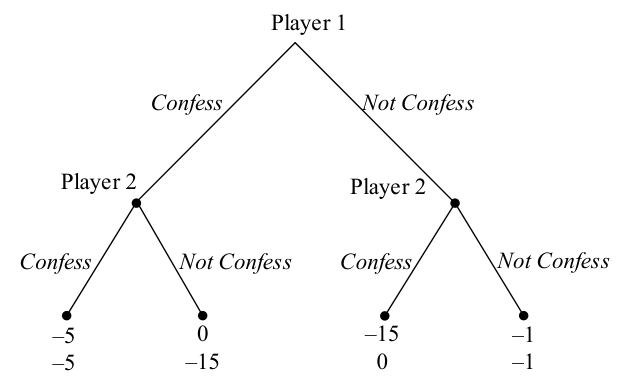
\includegraphics[width=0.55\linewidth]{figures/munoz-garcia-4-3.png}\\[2pt]
\small\textit{Fig.~4.9} Prisoner's dilemma sequential-move game
\end{center}
\begin{enumerate}[label=(\alph*),leftmargin=2em]
\item Find the best responses of the second mover, for each of the first mover's actions.
\item Find the first mover's equilibrium action and describe the subgame perfect Nash equilibrium of
the game.
\item Does the equilibrium behavior in the sequential-move game differ from its simultaneous-move
version?
\end{enumerate}

\begin{referencia}{``its simultaneous-move version'': Muñoz-Garcia \& Toro-Gonzalez (2019), Ch.~1,
Exercise 5 ``Prisoners' Dilemma Game'', Fig.~1.8, p.~9 [PDF 22]. Matrix rebuilt from the page.}
\jogo{Prisoner 1}{Prisoner 2}{\begin{tabular}{c|c|c|}
\hd{} & \hd{Confess} & \hd{Not confess}\\\cline{2-3}
Confess & -5, -5 & 0, -15\\\cline{2-3}
Not confess & -15, 0 & -1, -1\\\cline{2-3}
\end{tabular}}
\vspace{-6pt}\begin{center}\textit{Fig.~1.8} Normal-form of Prisoners' dilemma game\end{center}
\end{referencia}
\resolespaco

% ---------------------------------------------------------------------------
\exercicio[2]{Strategies and Equilibrium}{Foundations}{Tadelis (2013), \emph{Game Theory: An
Introduction}, Ch.~7 ``Preliminaries'', Exercise 7.2 ``Strategies and Equilibrium'', p.~147 [PDF
166]. No answer in the book. Reproduced verbatim.}

\rot{7.2}\textbf{Strategies and Equilibrium:} Consider a two-player game in which player 1 can
choose $A$ or $B$. The game ends if he chooses $A$ while it continues to player 2 if he chooses
$B$. Player 2 can then choose $C$ or $D$, with the game ending after $C$ and continuing again with
player 1 after $D$. Player 1 can then choose $E$ or $F$, and the game ends after each of these
choices.
\begin{partes}
\item Model this as an extensive-form game tree. Is it a game of perfect or imperfect information?
\item How many terminal nodes does the game have? How many information sets?
\item How many pure strategies does each player have?
\item Imagine that the payoffs following choice $A$ by player 1 are $(2, 0)$, those following $C$ by
player 2 are $(3, 1)$, those following $E$ by player 1 are $(0, 0)$, and those following $F$ by
player 1 are $(1, 2)$. What are the Nash equilibria of this game? Does one strike you as more
``appealing'' than the other? If so, explain why.
\end{partes}
\resolespaco

% ---------------------------------------------------------------------------
\exercicio[3]{Technology Adoption}{Exam level}{Tadelis (2013), \emph{Game Theory: An Introduction},
Ch.~8 ``Credibility and Sequential Rationality'', Exercise 8.5 ``Technology Adoption'', p.~170 [PDF
189]. No answer in the book. Reproduced verbatim.}

\rot{8.5}\textbf{Technology Adoption:} During the adoption of a new technology a CEO (player 1) can
design a new task for a division manager. The new task can be either high level ($H$) or low level
($L$). The manager simultaneously chooses to invest in good training ($G$) or bad training ($B$).
The payoffs from this interaction are given by the following matrix:
\jogo{Player 1}{Player 2}{\begin{tabular}{c|c|c|}
\hd{} & \hd{$G$} & \hd{$B$}\\\cline{2-3}
$H$ & 5, 4 & $-5$, 2\\\cline{2-3}
$L$ & 2, $-2$ & 0, 0\\\cline{2-3}
\end{tabular}}
\begin{partes}
\item Present the game in extensive form (a game tree) and solve for all the Nash equilibria and
subgame-perfect equilibria.
\item Now assume that before the game is played the CEO can choose not to adopt this new technology,
in which case the payoffs are (1, 1), or to adopt it, in which case the game is played. Present the
\emph{entire} game in extensive form. How many proper subgames does it have?
\item Solve for all the Nash equilibria and subgame-perfect equilibria of the game described in (b).
\end{partes}
\resolespaco

% ---------------------------------------------------------------------------
\exercicio[3]{Playing It Safe}{Exam level}{Tadelis (2013), \emph{Game Theory: An Introduction}, Ch.~8
``Credibility and Sequential Rationality'', Exercise 8.10 ``Playing It Safe'', p.~172 [PDF 191]. No
answer in the book. Reproduced verbatim.}

\rot{8.10}\textbf{Playing It Safe:} Consider the following dynamic game: Player 1 can choose to play
it safe (denote this choice by $S$), in which case both he and player 2 get a payoff of 3 each, or he
can risk playing a game with player 2 (denote this choice by $R$). If he chooses $R$ then they play
the following simultaneous-move game:
\jogo{Player 1}{Player 2}{\begin{tabular}{c|c|c|}
\hd{} & \hd{$A$} & \hd{$B$}\\\cline{2-3}
$C$ & 8, 0 & 0, 2\\\cline{2-3}
$D$ & 6, 6 & 2, 2\\\cline{2-3}
\end{tabular}}
\begin{partes}
\item Draw a game tree that represents this game. How many proper subgames does it have?
\item Are there other game trees that would work? Explain briefly.
\item Construct the matrix representation of the normal form of this dynamic game.
\item Find all the Nash and subgame-perfect equilibria of the dynamic game.
\end{partes}
\resolespaco

% ---------------------------------------------------------------------------
\exercicio[3]{Centipedes}{Exam level}{Tadelis (2013), \emph{Game Theory: An Introduction}, Ch.~7
``Preliminaries'', Exercise 7.4 ``Centipedes'', p.~148 [PDF 167]. No answer in the book.
Reproduced verbatim.}

\rot{7.4}\textbf{Centipedes:} Imagine a two-player game that proceeds as follows. A pot of money is
created with \$6 in it initially. Player 1 moves first, then player 2, then player 1 again, and
finally player 2 again. At each player's turn to move, he has two possible actions: grab ($G$) or
share ($S$). If he grabs he gets $\frac{2}{3}$ of the current pot of money, the other player gets
$\frac{1}{3}$ of the pot, and the game ends. If he shares then the size of the current pot is
multiplied by $\frac{3}{2}$ and the next player gets to move. At the last stage at which player 2
moves, if he chooses $S$ then the pot is still multiplied by $\frac{3}{2}$, player 2 gets
$\frac{1}{3}$ of the pot, and player 1 gets $\frac{2}{3}$ of the pot.
\begin{partes}
\item Model this as an extensive-form game tree. Is it a game of perfect or imperfect information?
\item How many terminal nodes does the game have? How many information sets?
\item How many pure strategies does each player have?
\item Find the Nash equilibria of this game. How many outcomes can be supported in equilibrium?
\item Now imagine that at the last stage at which player 2 moves, if he chooses to share then the
pot is equally split among the players. Does your answer to part (d) change?
\end{partes}
\resolespaco

% ---------------------------------------------------------------------------
\exercicio[4]{The Dean's Dilemma}{Exam level}{Tadelis (2013), \emph{Game Theory: An Introduction},
Ch.~7 ``Preliminaries'', Exercise 7.9 ``The Dean's Dilemma'', pp.~149--150 [PDF 168--169]. No
answer in the book. Reproduced verbatim.}

\rot{7.9}\textbf{The Dean's Dilemma:} A student stole the DVD player from the student lounge. The dean
of students (player 1) suspects the student (player 2) and begins collecting evidence. However,
evidence collection is a random process, and concrete evidence will be available to the dean only
with probability $\frac{1}{2}$. The student knows that the evidence-gathering process is under way
but does not know whether the dean has collected evidence or not. The game proceeds as follows: The
dean realizes whether or not he has evidence and can then choose his action, whether to accuse the
student ($A$) or bounce the case ($B$) and forget it. Once accused, the student has two options: he
can either confess ($C$) or deny ($D$). Payoffs are realized as follows: If the dean bounces the case
then both players get 0. If the dean accuses the student and the student confesses, the dean gains
2 and the student loses 2. If the dean accuses the student and the student denies, then payoffs
depend on the evidence: If the dean has no evidence then he loses face, which gives him a loss of
4, while the student gains glory, which gives him a payoff of 4. If, however, the dean has evidence
then he is triumphant and gains 4, while the student is put on probation and loses 4.
\begin{partes}
\item Draw the game tree that represents the extensive form of this game.
\item Write down the matrix that represents the normal form of the extensive form you drew in (a).
\item Solve for the Nash equilibria of the game.
\end{partes}
\resolespaco

% ---------------------------------------------------------------------------
\exercicio[4]{Perfect and Imperfect Recall}{Exam level}{Tadelis (2013), \emph{Game Theory: An
Introduction}, Ch.~7 ``Preliminaries'', Exercise 7.10 ``Perfect and Imperfect Recall'', p.~150 [PDF
169]. No answer in the book. Reproduced verbatim; Figure 7.14 cropped from the page.}

\rot{7.10}\textbf{Perfect and Imperfect Recall:} Consider the game depicted in Figure 7.14.
\begin{center}
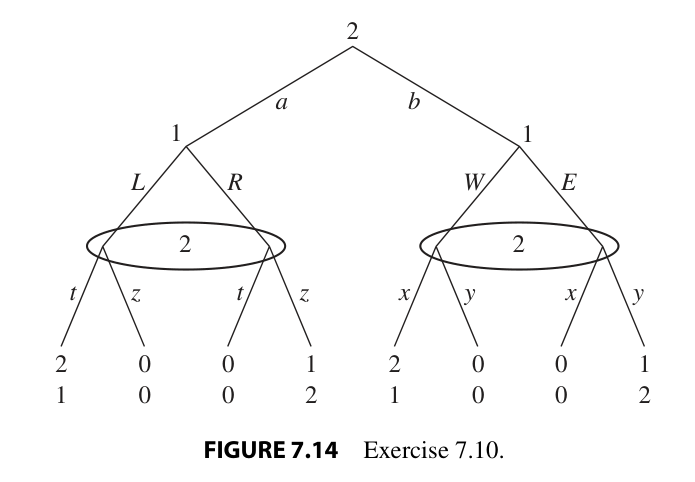
\includegraphics[width=0.6\linewidth]{figures/tadelis-7-10.png}
\end{center}
\begin{partes}
\item What are the pure-strategy sets for each player?
\item Show that for any behavioral strategy for player 1 there is a mixed strategy that leads to the
same distribution over the terminal nodes regardless of the strategy chosen by player 2.
\item Show that for any behavioral strategy for player 2 there is a mixed strategy that leads to the
same distribution over the terminal nodes regardless of the strategy chosen by player 1.
\item Now imagine that the game does not have perfect recall so that player 2's bottom two
information sets are now one large information set. Can you find an example showing that the claim
in (c) is no longer true?
\end{partes}
\resolespaco

% ---------------------------------------------------------------------------
\exercicio[4]{Zero-sum games of perfect information}{Advanced}{Mas-Colell, Whinston \& Green (1995),
\emph{Microeconomic Theory}, Ch.~9 ``Dynamic Games'', Exercises, Exercise 9.B.4$^{\mathrm{B}}$,
p.~302 [PDF 162, left half]. Answer in the MWG solutions manual (\texttt{Livros/}). Reproduced
verbatim.}

\rot{9.B.4$^{\mathrm{B}}$}Prove that in a finite \emph{zero-sum} game of perfect information, there
are unique subgame perfect Nash equilibrium payoffs.
\resolespaco

% ---------------------------------------------------------------------------
\exercicio[5]{The Rotten Kid Theorem}{Advanced}{Gibbons (1992), \emph{Game Theory for Applied
Economists}, Ch.~2 ``Dynamic Games of Complete Information'', \S2.6 Problems (Section 2.1),
Problem 2.1, p.~130 [PDF 137]. No answer in the book. Reproduced verbatim.}

\rot{2.1.}Suppose a parent and child play the following game, first analyzed by Becker (1974).
First, the child takes an action, $A$, that produces income for the child, $I_C(A)$, and income for
the parent, $I_P(A)$. (Think of $I_C(A)$ as the child's income net of any costs of the action $A$.)
Second, the parent observes the incomes $I_C$ and $I_P$ and then chooses a bequest, $B$, to leave to
the child. The child's payoff is $U(I_C + B)$; the parent's is $V(I_P - B) + kU(I_C + B)$, where
$k > 0$ reflects the parent's concern for the child's well-being. Assume that: the action is a
nonnegative number, $A \ge 0$; the income functions $I_C(A)$ and $I_P(A)$ are strictly concave and
are maximized at $A_C > 0$ and $A_P > 0$, respectively; the bequest $B$ can be positive or negative;
and the utility functions $U$ and $V$ are increasing and strictly concave. Prove the ``Rotten Kid''
Theorem: in the backwards-induction outcome, the child chooses the action that maximizes the
family's aggregate income, $I_C(A) + I_P(A)$, even though only the parent's payoff exhibits
altruism.
\resolespaco


\newpage
% Block 4 of lista-reais-lectures-01-05 (input by the drivers in Listas/).
% Order and ratings: lista-reais-lectures-01-05/order.md.
\bloco{4}{Credible threats and subgame perfection}{Lecture 4}

% ---------------------------------------------------------------------------
\exercicio[1]{Repeated-game definitions}{Foundations}{Gibbons (1992), \emph{Game Theory for Applied
Economists}, Ch.~2 ``Dynamic Games of Complete Information'', \S2.6 Problems (Section 2.3), Problem
2.12, p.~135 [PDF 142]. No answer in the book. Reproduced verbatim.}

\rot{2.12.}What is a strategy in a repeated game? What is a subgame in a repeated game? What is a
subgame-perfect Nash equilibrium?
\resolespaco

% ---------------------------------------------------------------------------
\exercicio[1]{Entering an Industry}{Foundations}{Tadelis (2013), \emph{Game Theory: An Introduction},
Ch.~7 ``Preliminaries'', Exercise 7.6 ``Entering an Industry'', pp.~148--149 [PDF 167--168]. No
answer in the book. Reproduced verbatim.}

\rot{7.6}\textbf{Entering an Industry:} A firm (player 1) is considering entering an established
industry with one incumbent firm (player 2). Player 1 must choose whether or not to enter the
industry. If player 1 enters the industry then player 2 can either accommodate the entry or fight
the entry by waging a price war. Player 1's most-preferred outcome is entering with player 2 not
fighting, and its least-preferred outcome is entering with player 2 fighting. Player 2's
most-preferred outcome is player 1 not entering, and its least-preferred outcome is player 1
entering with player 2 fighting.
\begin{partes}
\item Model this as an extensive-form game tree (choose payoffs that represent the preferences).
\item How many pure strategies does each player have?
\item Find all the Nash equilibria of this game.
\end{partes}
\resolespaco

% ---------------------------------------------------------------------------
\exercicio[2]{Entry Deterrence 1}{Foundations}{Tadelis (2013), \emph{Game Theory: An Introduction},
Ch.~8 ``Credibility and Sequential Rationality'', Exercise 8.8 ``Entry Deterrence 1'',
pp.~171--172 [PDF 190--191]. No answer in the book. Reproduced verbatim.}

\rot{8.8}\textbf{Entry Deterrence 1:} NSG Corporation is considering entry into the local phone
market in the San Francisco Bay Area. The incumbent, S\&P Corporation, predicts that a price war
will result if NSG enters. If NSG stays out, S\&P earns monopoly profits valued at \$10 million (net
present value of profits) while NSG earns zero. If NSG enters, it must incur irreversible entry
costs of \$2 million. If there is a price war, each firm earns \$1 million. S\&P always has the
option of accommodating entry (i.e., not starting a price war). In such a case both firms earn \$4
million (net present value). Suppose that the timing is such that NSG first has to choose whether or
not to enter the market. Then S\&P decides whether to ``accommodate entry'' or ``engage in a price
war.'' What is the subgame-perfect equilibrium outcome to this sequential game? Set up a game tree.
\resolespaco

% ---------------------------------------------------------------------------
\exercicio[3]{Investment in the Future}{Exam level}{Tadelis (2013), \emph{Game Theory: An
Introduction}, Ch.~8 ``Credibility and Sequential Rationality'', Exercise 8.6 ``Investment in the
Future'', pp.~170--171 [PDF 189--190]. No answer in the book. Reproduced verbatim.}

\rot{8.6}\textbf{Investment in the Future:} Consider two firms that play a Cournot competition game
with demand $p = 100 - q$ and costs for each firm given by $c_i(q_i) = 10q_i$. Imagine that before
the two firms play the Cournot game firm 1 can invest in cost reduction. If it invests the costs of
firm 1 will drop to $c_1(q_1) = 5q_1$. The cost of investment is $F > 0$. Firm 2 does not have this
investment opportunity.
\begin{partes}
\item Find the value $F^*$ for which the unique subgame-perfect equilibrium involves firm 1
investing.
\item Assume that $F > F^*$. Find a Nash equilibrium of the game that is not subgame perfect.
\end{partes}
\resolespaco

% ---------------------------------------------------------------------------
\exercicio[3]{Stackelberg with Two Firms}{Exam level}{Muñoz-Garcia \& Toro-Gonzalez (2019),
\emph{Strategy and Game Theory: Practice Exercises with Answers}, 2nd ed., Ch.~4
``Sequential-Move Games with Complete Information'', Exercise 11 ``Stackelberg with Two
Firms''$^{\mathrm{A}}$, p.~180 [PDF 192]. Worked answer in the book, right after the statement.
Reproduced verbatim (statement only).}

Consider a leader and a follower in a Stackelberg game of quantity competition. Firms face an
inverse demand curve $p(Q) = 1 - Q$, where $Q = q_L + q_F$ denotes aggregate output. The leader faces
a constant marginal cost $c_L > 0$ while the follower's constant marginal cost is $c_F > 0$, where
$1 > c_F \ge c_L$, indicating that the leader has access to a more efficient technology than the
follower.

\textbf{Part (a)} Find the follower's best response function, $BRF_F$, i.e., $q_F(q_L)$.

\textbf{Part (b)} Determine each firm's output strategy in the subgame perfect equilibrium (SPNE) of
this sequential-move game.

\textbf{Part (c)} Under which conditions on $c_L$ can you guarantee that both firms produce strictly
positive output levels?

\textbf{Part (d)} Assuming cost symmetry, i.e., $c_L = c_F = c$, determine the aggregate equilibrium
output level in the Stackelberg game, and its associated equilibrium price. Then compare them with
those arising in (1) a monopoly; in (2) the Cournot game of quantity competition; and (3) in the
Bertrand game of price competition (which, under cost symmetry, is analogous to a perfectly
competitive industry) [\emph{Hint}: For a more direct and visual comparison, depict the inverse
demand curve $p(Q) = 1 - Q$, and locate each of these four aggregate output levels in the horizontal
axis (with its associated prices in the vertical axis).].
\resolespaco

% ---------------------------------------------------------------------------
\exercicio[3]{Resident Assistant Selection with a Twist}{Exam level}{Tadelis (2013), \emph{Game Theory:
An Introduction}, Ch.~8 ``Credibility and Sequential Rationality'', Exercise 8.11 ``Resident
Assistant Selection with a Twist'', pp.~172--173 [PDF 191--192]. No answer in the book. Reproduced
verbatim.}

\rot{8.11}\textbf{Resident Assistant Selection with a Twist:} Two staff managers in the
$\Pi\mathrm{B}\Phi$ sorority, the house manager (player 1) and kitchen manager (player 2), must
select a resident assistant from a pool of three candidates: $\{a, b, c\}$. Player 1 prefers $a$ to
$b$, and $b$ to $c$. Player 2 prefers $b$ to $a$, and $a$ to $c$. The process that is imposed on them
is as follows: First, the house manager vetoes one of the candidates and announces the veto to the
central office for staff selection and to the kitchen manager. Next the kitchen manager vetoes one
of the remaining two candidates and announces it to the central office. Finally the director of the
central office assigns the remaining candidate to be a resident assistant at $\Pi\mathrm{B}\Phi$.
\begin{partes}
\item Model this as an extensive-form game (using a game tree) in which a player's most-preferred
candidate gives a payoff of 2, the second most-preferred candidate gives a payoff of 1, and the last
candidate gives 0.
\item Find the subgame-perfect equilibrium for this game. Is it unique?
\item Are there Nash equilibria that are not subgame-perfect equilibria?
\item Now assume that before the two players play the game, player 2 can send an alienating e-mail
to one of the candidates, which would result in that candidate withdrawing her application. Would
player 2 choose to do this, and if so, with which candidate?
\end{partes}
\resolespaco

% ---------------------------------------------------------------------------
\exercicio[4]{Industry Leader}{Exam level}{Tadelis (2013), \emph{Game Theory: An Introduction}, Ch.~8
``Credibility and Sequential Rationality'', Exercise 8.4 ``Industry Leader'', p.~170 [PDF 189]. No
answer in the book. Reproduced verbatim. (Gibbons Problem 2.6, p.~133, poses the same game and asks
only for the subgame-perfect outcome; it is not repeated in this list.)}

\rot{8.4}\textbf{Industry Leader:} Three oligopolists operate in a market with inverse demand given
by $P(Q) = a - Q$, where $Q = q_1 + q_2 + q_3$, and $q_i$ is the quantity produced by firm $i$. Each
firm has a constant marginal cost of production, $c$, and no fixed cost. The firms choose their
quantities dynamically as follows: Firm 1, which is the industry leader, chooses $q_1 \ge 0$. Firms
2 and 3 observe $q_1$ and then simultaneously choose $q_2$ and $q_3$, respectively.
\begin{partes}
\item How many proper subgames does this dynamic game have? Explain briefly.
\item Is it a game of perfect or imperfect information? Explain briefly.
\item What is the subgame-perfect equilibrium of this game? Show that it is unique.
\item Find a Nash equilibrium that is not a subgame-perfect equilibrium.
\end{partes}
\resolespaco

% ---------------------------------------------------------------------------
\exercicio[4]{Junk Mail Advertising}{Exam level}{Tadelis (2013), \emph{Game Theory: An Introduction},
Ch.~8 ``Credibility and Sequential Rationality'', Exercise 8.13 ``Junk Mail Advertising'',
pp.~173--174 [PDF 192--193]. No answer in the book. Reproduced verbatim.}

\rot{8.13}\textbf{Junk Mail Advertising:} Suppose a single good is owned by a single seller who
values it at $c > 0$ (he can consume the good and get a payoff of $c$). There is a single buyer who
has a small transportation cost $k > 0$ to get to and back from the seller's store, and he values
the good at $v > c + k$. The buyer first decides whether to make the commute or stay at home, not
buy the good, and receive a payoff of 0. If the buyer commutes to the store, the seller can then make
the buyer a take-it-or-leave-it price offer $p \ge 0$. The buyer can then accept the offer, pay $p$,
and get the good, or he can walk out and not buy the good. Assume that $c$, $v$, and $k$ are common
knowledge.
\begin{partes}
\item As best you can, draw the extensive form of this game. What is the best response of the buyer
at the node at which he decides whether to accept or reject the seller's offer?
\item Find the subgame-perfect equilibrium of the game and show that it is unique. Is it Pareto
optimal?
\item Are there Nash equilibria that yield a higher payoff to both players as compared to the
subgame-perfect equilibrium you found in (b)?
\item Now assume that before the game is played the seller can, at a small cost
$\varepsilon < (v - c - k)$, send the buyer a postcard that commits the seller to a certain price
at which the buyer can buy the good (e.g., ``bring this coupon and get the good at a price $p$'').
Would the seller choose to do so? Justify your answer with an equilibrium analysis.
\end{partes}
\resolespaco

% ---------------------------------------------------------------------------
\exercicio[4]{Debt and Repayment}{Advanced}{Tadelis (2013), \emph{Game Theory: An Introduction}, Ch.~8
``Credibility and Sequential Rationality'', Exercise 8.7 ``Debt and Repayment'', p.~171 [PDF 190].
No answer in the book. Reproduced verbatim.}

\rot{8.7}\textbf{Debt and Repayment:} A project costing \$100 yields a gross return of \$110. A
lender (player 1) is approached by a debtor (player 2) requesting a standard loan contract to
complete the project. If the lender chooses \emph{not to offer} a loan, then both parties earn
nothing. If the lender chooses to \emph{offer} a loan of \$100, the debtor can realize the project's
gains and is obliged by contract to repay \$105. For simplicity assume that money is continuous and
that the debtor can choose to return any amount of money $x \le 110$. Ignore the time value of
money. Assume first that no legal system is in place that can compel the debtor to repay, so that
default on the loan (less than full repayment) carries no repercussions for the debtor.
\begin{partes}
\item Model this as an extensive-form game tree as best you can and find a subgame-perfect
equilibrium of this game. Is it unique?
\item Now assume that there is a legal system in place that allows the lender to
\emph{voluntarily} choose whether or not to sue when the debtor defaults and repays an amount
$x < 105$. Furthermore assume that it is \emph{costless} to use the legal system (it is supplied by
the state), and if the lender sues a debtor that defaulted, the lender will get the \$105 repaid in
full. After paying the lender, the borrower will pay a fine of \$5 to the court, above and beyond
the repayment. Model this as an extensive-form game tree as best you can and find a subgame-perfect
equilibrium of this game. Is it unique?
\item Are there Nash equilibria in the game described in (b) that are not subgame-perfect
equilibria?
\item Now assume that using the legal system is \emph{costly:} if the lender sues, he pays lawyers a
\emph{legal fee} of \$105 (this is the lawyers' price; it is unrelated to the contract). The rest of
the game proceeds as before. (If the lender sues a debtor that defaulted, the lender will get repaid
in full; after paying the lender, the borrower will pay a fine of \$5 above and beyond the
repayment.) Model this as an extensive-form game tree as best you can and find a subgame-perfect
equilibrium of this game. Is it unique?
\item Are there Nash equilibria in the game described in (d) that are not subgame-perfect
equilibria?
\item Now assume that a change in the law is proposed: upon default, if a debtor is sued he has to
first repay the lender \$105 and then pay the legal fees of \$105 above and beyond repayment of the
loan, and no extra fine is imposed. Should the lender be willing to pay to have this change in the
law enacted? If so, how much?
\item If you were a social planner, would you implement the suggested law?
\end{partes}
\resolespaco

% ---------------------------------------------------------------------------
\exercicio[5]{Observation, multiple SPNE and moving first}{Advanced}{Mas-Colell, Whinston \& Green
(1995), \emph{Microeconomic Theory}, Ch.~9 ``Dynamic Games'', Exercises, Exercise
9.B.5$^{\mathrm{B}}$ (E.~Maskin), p.~302 [PDF 162, left half]. Answer in the MWG solutions manual
(\texttt{Livros/}; 9.B.5 is there). Reproduced verbatim; the label of the last part is blurred in
the scan and is read as (e), as in the solutions manual.}

\rot{9.B.5$^{\mathrm{B}}$}(E. Maskin) Consider a game with two players, player 1 and player 2, in
which each player $i$ can choose an action from a finite set $M_i$ that contains $m_i$ actions.
Player $i$'s payoff if the action choices are $(m_1, m_2)$ is $\phi_i(m_1, m_2)$.

\textbf{(a)} Suppose, first, that the two players move simultaneously. How many strategies does each
player have?

\textbf{(b)} Now suppose that player 1 moves first and that player 2 observes player 1's move before
choosing her move. How many strategies does each player have?

\textbf{(c)} Suppose that the game in (b) has multiple SPNEs. Show that if this is the case, then
there exist two pairs of moves $(m_1, m_2)$ and $(m_1', m_2')$ (where either $m_1 \neq m_1'$ or
$m_2 \neq m_2'$) such that either
\[ \text{(i)}\quad \phi_1(m_1, m_2) = \phi_1(m_1', m_2') \]
or
\[ \text{(ii)}\quad \phi_2(m_1, m_2) = \phi_2(m_1', m_2'). \]

\textbf{(d)} Suppose that for any two pairs of moves $(m_1, m_2)$ and $(m_1', m_2')$ such that
$m_1 \neq m_1'$ or $m_2 \neq m_2'$, condition (ii) is violated (i.e., player 2 is never indifferent
between pairs of moves). Suppose also that there exists a pure strategy Nash equilibrium in the
game in \textbf{(a)} in which $\pi_1$ is player 1's payoff. Show that in any SPNE of the game in
\textbf{(b)}, player 1's payoff is at least $\pi_1$. Would this conclusion necessarily hold for any
\emph{Nash} equilibrium of the game in \textbf{(b)}?

\textbf{(e)} Show by example that the conclusion in \textbf{(d)} may fail either if condition (ii)
holds for some strategy pairs $(m_1, m_2)$, $(m_1', m_2')$ with $m_1 \neq m_1'$ or
$m_2 \neq m_2'$ or if we replace the phrase \emph{pure strategy Nash equilibrium} with the phrase
\emph{mixed strategy Nash equilibrium}.
\resolespaco


\newpage
% Block 5 of lista-reais-lectures-01-05 (input by the drivers in Listas/).
% Order and ratings: lista-reais-lectures-01-05/order.md.
\bloco{5}{Repeated games and bargaining}{Lecture 5}

% ---------------------------------------------------------------------------
\exercicio[1]{Finitely repeated game}{Foundations}{Cabral (2017), \emph{Introduction to Industrial
Organization}, 2nd ed., Ch.~7 ``Games and Strategies'', Exercises, Exercise 7.13 ``Finitely repeated
game'', p.~182 [PDF 194]. No answer in the book. Reproduced verbatim.}

\rot{7.13.}\textbf{Finitely repeated game.} Suppose that the game depicted in Figure 7.1 is repeated
$T$ times, where $T$ is known. Show that the only subgame perfect equilibrium is for players to
choose $(B, R)$ in every period.

\begin{referencia}{``the game depicted in Figure 7.1'': Cabral (2017), Ch.~7, Figure 7.1 ``The
`prisoner's dilemma' game'' and the sentence that explains how its cells are read, p.~160 [PDF 172].
Figure cropped from the page; text reproduced verbatim.}
For each combination of strategies by each player, the respective matrix cell shows the payoffs
received by each player. In the lower left corner, the payoff received by Player 1; in the top right
corner, the payoff received by Player 2.
\begin{center}
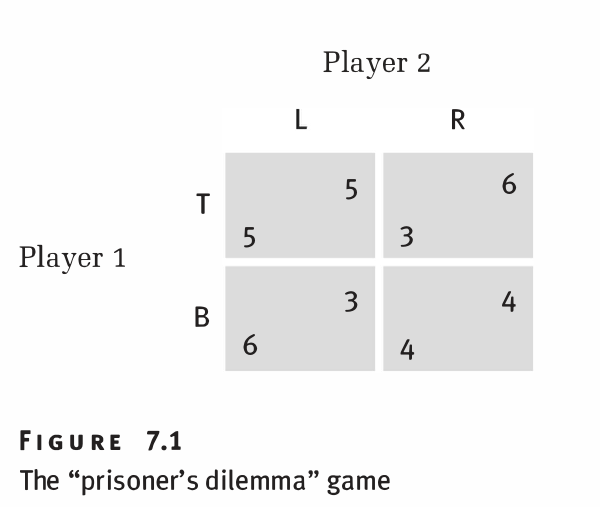
\includegraphics[width=0.42\linewidth]{figures/cabral-7-1.png}
\end{center}
\end{referencia}
\resolespaco

% ---------------------------------------------------------------------------
\exercicio[2]{Grim Trigger}{Foundations}{Tadelis (2013), \emph{Game Theory: An Introduction}, Ch.~10
``Repeated Games'', Exercise 10.2 ``Grim Trigger'', p.~215 [PDF 234]. No answer in the book.
Reproduced verbatim.}

\rot{10.2}\textbf{Grim Trigger:} Consider the infinitely repeated game with discount factor
$\delta < 1$ of the following variant of the Prisoner's Dilemma:
\jogo{Player 1}{Player 2}{\begin{tabular}{c|c|c|c|}
\hd{} & \hd{$L$} & \hd{$C$} & \hd{$R$}\\\cline{2-4}
$T$ & 6, 6 & $-1$, 7 & $-2$, 8\\\cline{2-4}
$M$ & 7, $-1$ & 4, 4 & $-1$, 5\\\cline{2-4}
$B$ & 8, $-2$ & 5, $-1$ & 0, 0\\\cline{2-4}
\end{tabular}}
\begin{partes}
\item For which values of the discount factor $\delta$ can the players support the pair of actions
$(M, C)$ played in every period?
\item For which values of the discount factor $\delta$ can the players support the pair of actions
$(T, L)$ played in every period? Why is your answer different from that for (a)?
\end{partes}
\resolespaco

% ---------------------------------------------------------------------------
\exercicio[2]{Infinitely Repeated Prisoner's Dilemma Game}{Foundations}{Muñoz-Garcia \& Toro-Gonzalez
(2019), \emph{Strategy and Game Theory: Practice Exercises with Answers}, 2nd ed., Ch.~6 ``Repeated
Games and Correlated Equilibria'', Exercise 1 ``Infinitely Repeated Prisoner's Dilemma
Game''$^{\mathrm{A}}$, p.~274 [PDF 285]. Worked answer in the book, right after the statement.
Reproduced verbatim (statement only); Table 6.1 rebuilt from the same page.}

Consider the infinitely repeated version of the following prisoner's dilemma game, where C denotes
confess and NC represents not confess (Table 6.1):

\textbf{Part (a)} Can players support the cooperative outcome (NC, NC) as a SPNE by using
tit-for-tat strategies, whereby players punish deviations from NC in a past period by reverting to
the stage-game Nash equilibrium where they both confess (C, C) for just one period, and then
returning to cooperation?

\textbf{Part (b)} Consider now that players play tit-for-tat, but reverting to the stage-game Nash
equilibrium where they both confess (C, C) for two periods, and then players return to cooperation.
Can the cooperative outcome (NC, NC) be supported as a SPNE?

\textbf{Part (c)} Suppose that players use strategies that punish deviation from cooperation by
reverting to the stage-game Nash equilibrium for ten periods before returning to cooperation.
Compute the threshold discount factor, $\delta$, above which cooperation can be sustained as a SPNE
of the infinitely repeated game.
\jogo{Player 1}{Player 2}{\begin{tabular}{c|c|c|}
\hd{} & \hd{C} & \hd{NC}\\\cline{2-3}
C & 2, 2 & 6, 0\\\cline{2-3}
NC & 0, 6 & 3, 3\\\cline{2-3}
\end{tabular}}
\vspace{-6pt}\begin{center}\small\textit{Table 6.1} Prisoner's dilemma game\end{center}
\resolespaco

% ---------------------------------------------------------------------------
\exercicio[3]{Representing Feasible, Individually Rational Payoffs}{Exam level}{Muñoz-Garcia \&
Toro-Gonzalez (2019), \emph{Strategy and Game Theory: Practice Exercises with Answers}, 2nd ed.,
Ch.~6 ``Repeated Games and Correlated Equilibria'', Exercise 9 ``Representing Feasible,
Individually Rational Payoffs''$^{\mathrm{C}}$, p.~305 [PDF 316]. Worked answer in the book, right
after the statement. Reproduced verbatim (statement only); Table 6.6, printed inside the answer on
the same page, rebuilt.}

Consider an infinitely-repeated game where the stage game is depicted Table 6.6. Player 1 chooses
rows and player 2 chooses columns. Players discount the future using a common discount factor
$\delta$.

\textbf{Part (a)} What outcomes in the stage-game are consistent with Nash equilibrium play?

\textbf{Part (b)} Let $v_1$ and $v_2$ be the repeated game payoffs to player 1 and player 2
respectively. Draw the set of feasible payoffs from the repeated game, explaining any normalization
you use.

\textbf{Part (c)} Find the set of individually rational feasible set of payoffs.

\textbf{Part (d)} Find a Nash equilibrium in which the players obtain (9, 9) each period. What
restrictions on $\delta$ are necessary?
\jogo{Player 1}{Player 2}{\begin{tabular}{c|c|c|}
\hd{} & \hd{$L$} & \hd{$R$}\\\cline{2-3}
$U$ & 9, 9 & 1, 10\\\cline{2-3}
$D$ & 10, 1 & 7, 7\\\cline{2-3}
\end{tabular}}
\vspace{-6pt}\begin{center}\small\textit{Table 6.6} Simultaneous-move game\end{center}
\resolespaco

% ---------------------------------------------------------------------------
\exercicio[3]{Not-So-Grim Trigger}{Exam level}{Tadelis (2013), \emph{Game Theory: An Introduction},
Ch.~10 ``Repeated Games'', Exercise 10.3 ``Not-So-Grim Trigger'', pp.~215--216 [PDF 234--235]. No
answer in the book. Reproduced verbatim, with the book's footnote 12 (p.~216). Here $T$ is the
length of the punishment.}

\rot{10.3}\textbf{Not-So-Grim Trigger:} Consider the infinitely repeated Prisoner's Dilemma with
discount factor $\delta < 1$ described by the following matrix:
\jogo{Player 1}{Player 2}{\begin{tabular}{c|c|c|}
\hd{} & \hd{$m$} & \hd{$f$}\\\cline{2-3}
$M$ & 4, 4 & $-1$, 5\\\cline{2-3}
$F$ & 5, $-1$ & 1, 1\\\cline{2-3}
\end{tabular}}
Instead of using grim-trigger strategies to support a pair of actions $(a_1, a_2)$ other than
$(F, f)$ as a subgame-perfect equilibrium, assume that the players wish to choose a less draconian
punishment called a ``length-$T$ punishment'' strategy. If there is a deviation from $(a_1, a_2)$
then the players will play $(F, f)$ for $T$ periods and then resume playing $(a_1, a_2)$. Let
$\delta_T$ be the critical discount factor so that if $\delta > \delta_T$ then the adequately
defined strategies will implement the desired path of play with length-$T$ punishment as the
threat.
\begin{partes}
\item Let $T = 1$. What is the critical value $\delta_1$ to support the pair of actions $(M, m)$
played in every period?
\item Let $T = 2$. What is the critical value $\delta_T$ to support the pair of actions $(M, m)$
played in every period?$^{12}$
\item Compare the two critical values in (a) and (b). How do they differ and what is the intuition
for this?
\end{partes}
{\small $^{12}$\,Hint: You should encounter an equation of the form $a\delta^3 - (a + 1)\delta + 1 = 0$,
for which it is easy to see that $\delta = 1$ is a root. In this case you know that the equation can
be written in the form $(\delta - 1)(a\delta^2 + a\delta - 1) = 0$, and you can solve for the other
relevant root of the cubic equation.\par}
\resolespaco

% ---------------------------------------------------------------------------
\exercicio[4]{Multistage Practice}{Exam level}{Tadelis (2013), \emph{Game Theory: An Introduction},
Ch.~9 ``Multistage Games'', Exercise 9.1 ``Multistage Practice'', pp.~186--187 [PDF 205--206]. No
answer in the book. Reproduced verbatim.}

\rot{9.1}\textbf{Multistage Practice:} Consider the following simultaneous-move game that is played
twice (the players observe the first-period outcome prior to the second-period play):
\jogo{Player 1}{Player 2}{\begin{tabular}{c|c|c|c|}
\hd{} & \hd{$L$} & \hd{$C$} & \hd{$R$}\\\cline{2-4}
$T$ & 10, 10 & 2, 12 & 0, 13\\\cline{2-4}
$M$ & 12, 2 & 5, 5 & 0, 0\\\cline{2-4}
$B$ & 13, 0 & 0, 0 & 1, 1\\\cline{2-4}
\end{tabular}}
\begin{partes}
\item Find all the pure-strategy subgame-perfect equilibria with no discounting ($\delta = 1$). Be
precise in defining history-contingent strategies for both players.
\item For each of the equilibria you found in (a), find the smallest discount factor that supports
it.
\end{partes}
\resolespaco

% ---------------------------------------------------------------------------
\exercicio[4]{Reaching a non-Nash payoff in the first stage}{Exam level}{Gibbons (1992), \emph{Game
Theory for Applied Economists}, Ch.~2 ``Dynamic Games of Complete Information'', \S2.6 Problems
(Section 2.3), Problem 2.11, p.~135 [PDF 142]. No answer in the book (Muñoz-Garcia \&
Toro-Gonzalez Ch.~6 Ex.~7, p.~299, works the same game). Reproduced verbatim.}

\rot{2.11.}The simultaneous-move game (below) is played twice, with the outcome of the first stage
observed before the second stage begins. There is no discounting. Can the payoff $(4, 4)$ be achieved
in the first stage in a pure-strategy subgame-perfect Nash equilibrium? If so, give strategies that
do so. If not, prove why not.
\begin{center}\begin{tabular}{c|c|c|c|}
\hd{} & \hd{$L$} & \hd{$C$} & \hd{$R$}\\\cline{2-4}
$T$ & 3, 1 & 0, 0 & 5, 0\\\cline{2-4}
$M$ & 2, 1 & 1, 2 & 3, 1\\\cline{2-4}
$B$ & 1, 2 & 0, 1 & 4, 4\\\cline{2-4}
\end{tabular}\end{center}
\resolespaco

% ---------------------------------------------------------------------------
\exercicio[4]{Asymmetric Patience 1}{Exam level}{Tadelis (2013), \emph{Game Theory: An Introduction},
Ch.~11 ``Strategic Bargaining'', Exercise 11.5 ``Asymmetric Patience 1'', pp.~236--237 [PDF
255--256]. No answer in the book. Reproduced verbatim.}

\rot{11.5}\textbf{Asymmetric Patience 1:} Consider a three-period sequential (alternating-offer)
bargaining model in which two players have to split a pie worth 1 (starting with player 1 making
the offer). Now the players have different discount factors, $\delta_1$ and $\delta_2$.
\begin{partes}
\item Compute the outcome of the unique subgame-perfect equilibrium.
\item Show that when $\delta_1 = \delta_2$ player 1 has an advantage.
\item What conditions on $\delta_1$ and $\delta_2$ give player 2 an advantage? Why?
\end{partes}

\begin{referencia}{the alternating-offer bargaining model this exercise modifies (``Now the
players have different discount factors''): Tadelis (2013), Ch.~11 ``Strategic Bargaining'',
p.~221 [PDF 240]. Reproduced verbatim (excerpts); with $\delta_1 \neq \delta_2$, player $i$
discounts with $\delta_i$.}
In the first round:
\begin{itemize}[leftmargin=1.6em]
\item Player 1 offers shares $(x, 1 - x)$, where player 1 receives $x$ and player 2 receives $1 - x$.
\item Player 2 then chooses to accept, causing the game to end with payoffs $v_1 = x$ and
$v_2 = 1 - x$, or reject, causing the game to move to the second round.
\end{itemize}
In the second round:
\begin{itemize}[leftmargin=1.6em]
\item A share $1 - \delta$ of the pie is dissipated (the pie is discounted with discount factor
$0 < \delta < 1$).
\item Player 2 offers shares $(x, 1 - x)$, where player 1 receives $x$ and player 2 receives $1 - x$.
\item Player 1 chooses to accept, causing the game to end with payoffs $v_1 = \delta x$ and
$v_2 = \delta(1 - x)$, or reject, causing the game to move to the third round.
\end{itemize}
In the third round and beyond:
\begin{itemize}[leftmargin=1.6em]
\item The game continues in the same way, where following rejection in an odd period player 2 gets
to offer in the next even period, and vice versa.
\item Each period has further discounting of the pie, so that in period $t$ the total pie is worth
$\delta^{t-1}$.
\end{itemize}
[\ldots] Assume for now that the game ends in some prespecified final period $T$, which will be
reached if the players did not reach an agreement in the $T - 1$ periods that preceded $T$.
Furthermore assume that period $T$ is a ``hard deadline,'' so that both players receive a payoff of
zero if they fail to reach an agreement in this last period.
\end{referencia}
\resolespaco

% ---------------------------------------------------------------------------
\exercicio[4]{Diluted Happiness}{Advanced}{Tadelis (2013), \emph{Game Theory: An Introduction}, Ch.~10
``Repeated Games'', Exercise 10.7 ``Diluted Happiness'', pp.~217--218 [PDF 236--237]. No answer in
the book. Reproduced verbatim.}

\rot{10.7}\textbf{Diluted Happiness:} Consider a relationship between a bartender and a customer. The
bartender serves bourbon to the customer and chooses $x \in [0, 1]$, which is the proportion of
bourbon in the drink served, while $1 - x$ is the proportion of water. The cost of supplying such a
drink (standard 4-ounce glass) is $cx$, where $c > 0$. The customer, without knowing $x$, decides on
whether or not to buy the drink at the market price $p$. If he buys the drink his payoff is
$vx - p$, and the bartender's payoff is $p - cx$. Assume that $v > c$ and all payoffs are common
knowledge. If the customer does not buy the drink he gets 0 and the bartender gets $-cx$. Because
the customer has some experience, once the drink is bought and he tastes it, he learns the value of
$x$, but this is only after he pays for the drink.
\begin{partes}
\item Find all the Nash equilibria of this game.
\item Now assume that the customer is visiting town for 10 days, and this ``bar game'' will be
played on each of the 10 evenings that the customer is in town. Assume that each player tries to
maximize the (nondiscounted) sum of his stage payoffs. Find all the subgame-perfect equilibria of
this game.
\item Now assume that the customer is a local, and the players perceive the game as repeated
infinitely many times. Assume that each player tries to maximize the discounted sum of his stage
payoffs, where the discount rate is $\delta \in (0, 1)$. What is the range of prices $p$ (expressed
in the parameters of the problem) for which there exists a subgame-perfect equilibrium in which
every day the bartender chooses $x = 1$ and the customer buys at the price $p$?
\item For which values of $\delta$ (expressed in the parameters of the problem) can the price range
that you found in (c) exist?
\end{partes}
\resolespaco

% ---------------------------------------------------------------------------
\needspace{20\baselineskip}
\exercicio[5]{Rubinstein's strategies are subgame-perfect}{Advanced}{Gibbons (1992), \emph{Game Theory
for Applied Economists}, Ch.~2 ``Dynamic Games of Complete Information'', \S2.6 Problems (Section
2.4), Problem 2.20, pp.~137--138 [PDF 144--145]. No answer in the book. Reproduced verbatim.}

\rot{2.20.}Consider the following strategies in the infinite-horizon version of Rubinstein's
bargaining model. (Recall the notational convention that the offer $(s, 1 - s)$ means that Player 1
will get $s$ and Player 2 will get $1 - s$, independent of who made the offer.) Let
$s^* = 1/(1 + \delta)$. Player 1 always offers $(s^*, 1 - s^*)$ and accepts an offer $(s, 1 - s)$
only if $s \ge \delta s^*$. Player 2 always offers $(1 - s^*, s^*)$ and accepts an offer
$(s, 1 - s)$ only if $1 - s \ge \delta s^*$. Show that these strategies are a Nash equilibrium.
Show that this equilibrium is subgame-perfect.

\begin{referencia}{``the infinite-horizon version of Rubinstein's bargaining model'': Gibbons (1992),
\S2.1.D ``Sequential Bargaining'', pp.~68--70 [PDF 75--77]. Reproduced verbatim (excerpts); footnote~7
(on the discount factor as $\delta = 1/(1+r)$) omitted.}
Players 1 and 2 are bargaining over one dollar. They alternate in making offers: first player 1
makes a proposal that player 2 can accept or reject; if 2 rejects then 2 makes a proposal that 1 can
accept or reject; and so on. Once an offer has been rejected, it ceases to be binding and is
irrelevant to the subsequent play of the game. Each offer takes one period, and the players are
impatient: they discount payoffs received in later periods by the factor $\delta$ per period, where
$0 < \delta < 1$.

A more detailed description of the timing of the three-period bargaining game is as follows.
\begin{itemize}[leftmargin=2.6em]
\item[(1a)] At the beginning of the first period, player 1 proposes to take a share $s_1$ of the
dollar, leaving $1 - s_1$ for player 2.
\item[(1b)] Player 2 either accepts the offer (in which case the game ends and the payoffs $s_1$ to
player 1 and $1 - s_1$ to player 2 are immediately received) or rejects the offer (in which case
play continues to the second period).
\item[(2a)] At the beginning of the second period, player 2 proposes that player 1 take a share
$s_2$ of the dollar, leaving $1 - s_2$ for player 2. (Note the convention that $s_t$ always goes to
player 1, regardless of who made the offer.)
\item[(2b)] Player 1 either accepts the offer (in which case the game ends and the payoffs $s_2$ to
player 1 and $1 - s_2$ to player 2 are immediately received) or rejects the offer (in which case
play continues to the third period).
\item[(3)] At the beginning of the third period, player 1 receives a share $s$ of the dollar,
leaving $1 - s$ for player 2, where $0 < s < 1$.
\end{itemize}
[\ldots] Now consider the infinite-horizon case. The timing is as described previously, except that
the exogenous settlement in step (3) is replaced by an infinite sequence of steps (3a), (3b), (4a),
(4b), and so on. Player 1 makes the offer in odd-numbered periods, player 2 in even-numbered;
bargaining continues until one player accepts an offer.
\end{referencia}
\resolespaco


\end{document}
